% ---------
%  Compile with "pdflatex hw0".
% --------
%!TEX TS-program = pdflatex
%!TEX encoding = UTF-8 Unicode
%!TEX spellcheck = English (Aspell)

\documentclass[11pt]{article}
\usepackage{jeffe,handout,graphicx}
\usepackage{fourier-orns}
\usepackage{mathtools}

\def\Cdot{\mathbin{\text{\normalfont \textbullet}}}
\def\Sym#1{\texttt{\color{BrickRed}#1}}
\def\BlueSym#1{\textbf{\texttt{\color{RoyalBlue}#1}}}
\allowdisplaybreaks

% =========================================================
\begin{document}

\thispagestyle{empty}

\begin{center}
\Large\textbf{CS/ECE 374 A \,\decosix\, Fall 2023}%
\\
\LARGE\textbf{\decothreeleft~ Homework 1 ~\decothreeright}%
\\[0.5ex]
\large Due Tuesday, August 29, 2023 at 9pm Central Time
\end{center}

\bigskip
\hrule
\bigskip
\begin{itemize}

\item
\textbf{Submit your written solutions electronically to Gradescope as PDF files.}  Submit a separate PDF file for each numbered problem.  If you plan to typeset your solutions, you are welcome to use the \LaTeX\ solution template on the course web site.  If you must submit scanned handwritten solutions, please use a black pen on blank white paper and a high-quality scanner app (or an actual scanner).

\item
Groups of up to three people can submit joint solutions on Gradescope.  \EMPH{Exactly} one student in each group should upload the solution and indicate their other group members.

\item
\textbf{You may use any source at your disposal}—paper, electronic,\footnote{Yes, including ChatGPT.} or human—but you \EMPH{must} cite \EMPH{every} source that you use,\footnote{Yes, including ChatGPT.} you \EMPH{must} write everything yourself in your own words, and you are responsible for any errors in the sources you use.\footnote{Yes, including ChatGPT.}  See the academic integrity policies on the course web site for more details. 

\item
Written homework is normally due every Tuesday at 9pm.  In addition, guided problem sets on PrairieLearn are normally due every \textbf{Monday} at 9pm; each student must do these individually.  In particular, Guided Problem Set 1 is due Monday, August 28!  

\item
Both guided problem sets and homework may be submitted up to 24 hours late for 50\% partial credit, or for full credit with an approved extension. See the grading policies on the course web site for more details.

\item
Each homework will include at least one fully solved problem, similar to that week’s   assigned problems, together with the rubric we would use to grade this problem if it appeared in an actual homework or exam.  These model solutions show our recommendations for structure, presentation, and level of detail in your homework solutions.  (Obviously, the actual \emph{content} of your solutions won’t match the model solutions, because your problems are different!)  Homeworks may also include additional practice problems.

\item
Standard grading rubrics for many problem types can be found on the course web page.   For example, the problems in this week’s homework will be graded using the standard induction rubric.  (Weak induction makes the baby Jesus cry.)


\end{itemize}

\bigskip
\hrule
\smallskip

\begin{center}
\large \textbf{See the course web site for more information.}\\[1ex]\normalsize
If you have any questions about these policies,\\
please don’t hesitate to ask in class, in office hours, or on Piazza.
\end{center}

\hrule

%----------------------------------------------------------------------
\headers{CS/ECE 374 A}{Homework 1 (due August 29)}{Fall 2023}

\begin{enumerate}
%\parindent 1.5em \itemsep 4ex plus 0.5fil

%----------------------------------------------------------------------
\item
Consider the following recursively defined function:
\[
	\emph{stutter}(w) := \begin{cases}
		\e & \text{if $w=\e$}\\[0.25ex]
		aa\Cdot \emph{stutter}(x) & \text{if $w = ax$}
	\end{cases}
\]
For example, $\emph{stutter}(\Sym{MISSISSIPPI}) = \Sym{MMIISSSSIISSSSIIPPPPII}$.
\begin{enumerate}
\item
Prove that $\abs{\emph{stutter}(w)} = 2\abs{w}$ for every string $w$.

\item
Prove that $\emph{stutter}(x\Cdot y) = \emph{stutter}(x)\Cdot \emph{stutter}(y)$ for all strings $x$ and $y$.

\item
\textcolor{PineGreen}{\EMPH{\textul{Practice only. Do not submit solutions.}}}

The \EMPH{reversal $w^R$} of a string $w$ is defined recursively as follows:
\[	
	w^R := \begin{cases}
		\e & \text{if $w=\e$} \\[0.5ex]
		x^R \Cdot a & \text{if $w=ax$}
	\end{cases}
\]
For example, $\Sym{MISSIPPIPPI}^R = \Sym{IPPIPPISSIM}$.

Prove that $\emph{stutter}(w)^R = \emph{stutter}(w^R)$ for every string $w$.

\end{enumerate}

You may freely use any result proved in lecture, in lab, or in the lecture notes.  Otherwise your proofs must be formal and self-contained.  In particular, your proofs \emph{must} invoke the formal recursive definitions of string length and concatenation \textcolor{PineGreen}{(and for part (c), reversal)}.

%----------------------------------------------------------------------
\newpage
\item
For each positive integer $n$, we define two strings $p_n$ and $v_n$, respectively called the $n$th \emph{Piṅgala string} and the $n$th \emph{Virahāṇka string}.  Piṅgala strings are defined by the following recurrence:
\[
	p_n = \begin{cases}
		\Sym1 & \text{if $n=1$} \\
		\Sym0 & \text{if $n=2$} \\
		p_{n-2}\Cdot p_{n-1} & \text{otherwise}
	\end{cases}
\]
For example:
\[
	p_7
	= \overbracket[0.75pt]{\Sym{10010}}^{p_5}
		\overbracket[0.75pt]{
			\overbracket[0.75pt]{\Sym{010}}^{p_4}
			\overbracket[0.75pt]{\Sym{10010}}^{p_5}
		}^{p_6}.
\]

Virahāṇka strings are defined more indirectly as 
\[
	v_n = \begin{cases}
		\Sym1 & \text{if $n=1$} \\
		\textsf{grow}(v_{n-1}) & \text{otherwise}
	\end{cases}
\]
where the string function \textsf{grow} is defined as follows:
\[
	\textsf{grow}(w) = 
	\begin{cases}
		\e & \text{if $w = \e$} \\
		\Sym0\cdot \textsf{grow}(x) & \text{if $w = \Sym1 x$} \\
		\Sym{10}\Cdot \textsf{grow}(x) & \text{if $w = \Sym0 x$}
	\end{cases}
\]
For example:
\[
	\textsf{grow}(\Sym{01010010})
	=
	\Sym{10}\Cdot \Sym0\Cdot \Sym{10}\Cdot \Sym0\Cdot \Sym{10}\Cdot \Sym{10}\Cdot \Sym0\Cdot \Sym{10} 
	=
	\Sym{1001001010010}
\]
Finally, recall that the Fibonacci numbers are defined recursively as follows:
\[
	F_n = \begin{cases}
		0 & \text{if $n=0$} \\
		1 & \text{if $n=1$} \\
		F_{n-1}+F_{n-2} & \text{otherwise}
	\end{cases}
\]

\begin{enumerate}
\item
Prove that $\abs{p_n} = F_n$ for all $n\ge 1$.

\item
Prove that $\textsf{grow}(w\Cdot z) = \textsf{grow}(w) \Cdot \textsf{grow}(z)$ for all strings $w$ and $z$.

\item
Prove that $p_n = v_n$ for all $n \ge 1$.  \Hint{Careful!}

\item
\textcolor{PineGreen}{\EMPH{\textul{Practice only. Do not submit solutions.}}}

Prove that $\abs{v_n} = F_n$ for all $n\ge 1$.
\end{enumerate}

As in problem 1, you may freely use any result that proved in lecture, in lab, or in the lecture notes.  Otherwise your proofs must be formal and self-contained.  In particular, your proofs \emph{must} invoke the formal recursive definitions of the strings $p_n$ and $v_n$, the \textsf{grow} function, and the Fibonacci numbers $F_n$.



%----------------------------------------------------------------------
\newpage
\Hard
\item
\textcolor{PineGreen}{\EMPH{\textul{Practice only. Do not submit solutions.}}}

For each non-negative integer $n$, we recursively define two binary trees $P_n$ and $V_n$, called the $n$th \emph{Piṅgala tree} and the $n$th \emph{Virahāṇka tree}, respectively.

\begin{itemize}
\item
$P_0$ and $V_0$ are empty trees, with no nodes.
\item
$P_1$ and $V_1$ each consist of a single node.
\item 
For any integer $n\ge 2$, the tree $P_n$ consists of a root with two subtrees; the left subtree is a copy of $P_{n-1}$, and the right subtree is a copy of $P_{n-2}$.
\item
For any integer $n\ge 2$, the tree $L_n$ is obtained from $L_{n-1}$ by attaching a new right child to every leaf and attaching a new left child to every node that has only a right child.
\end{itemize}
The following figure shows the recursive construction of these two trees when $n=7$.
\begin{center}
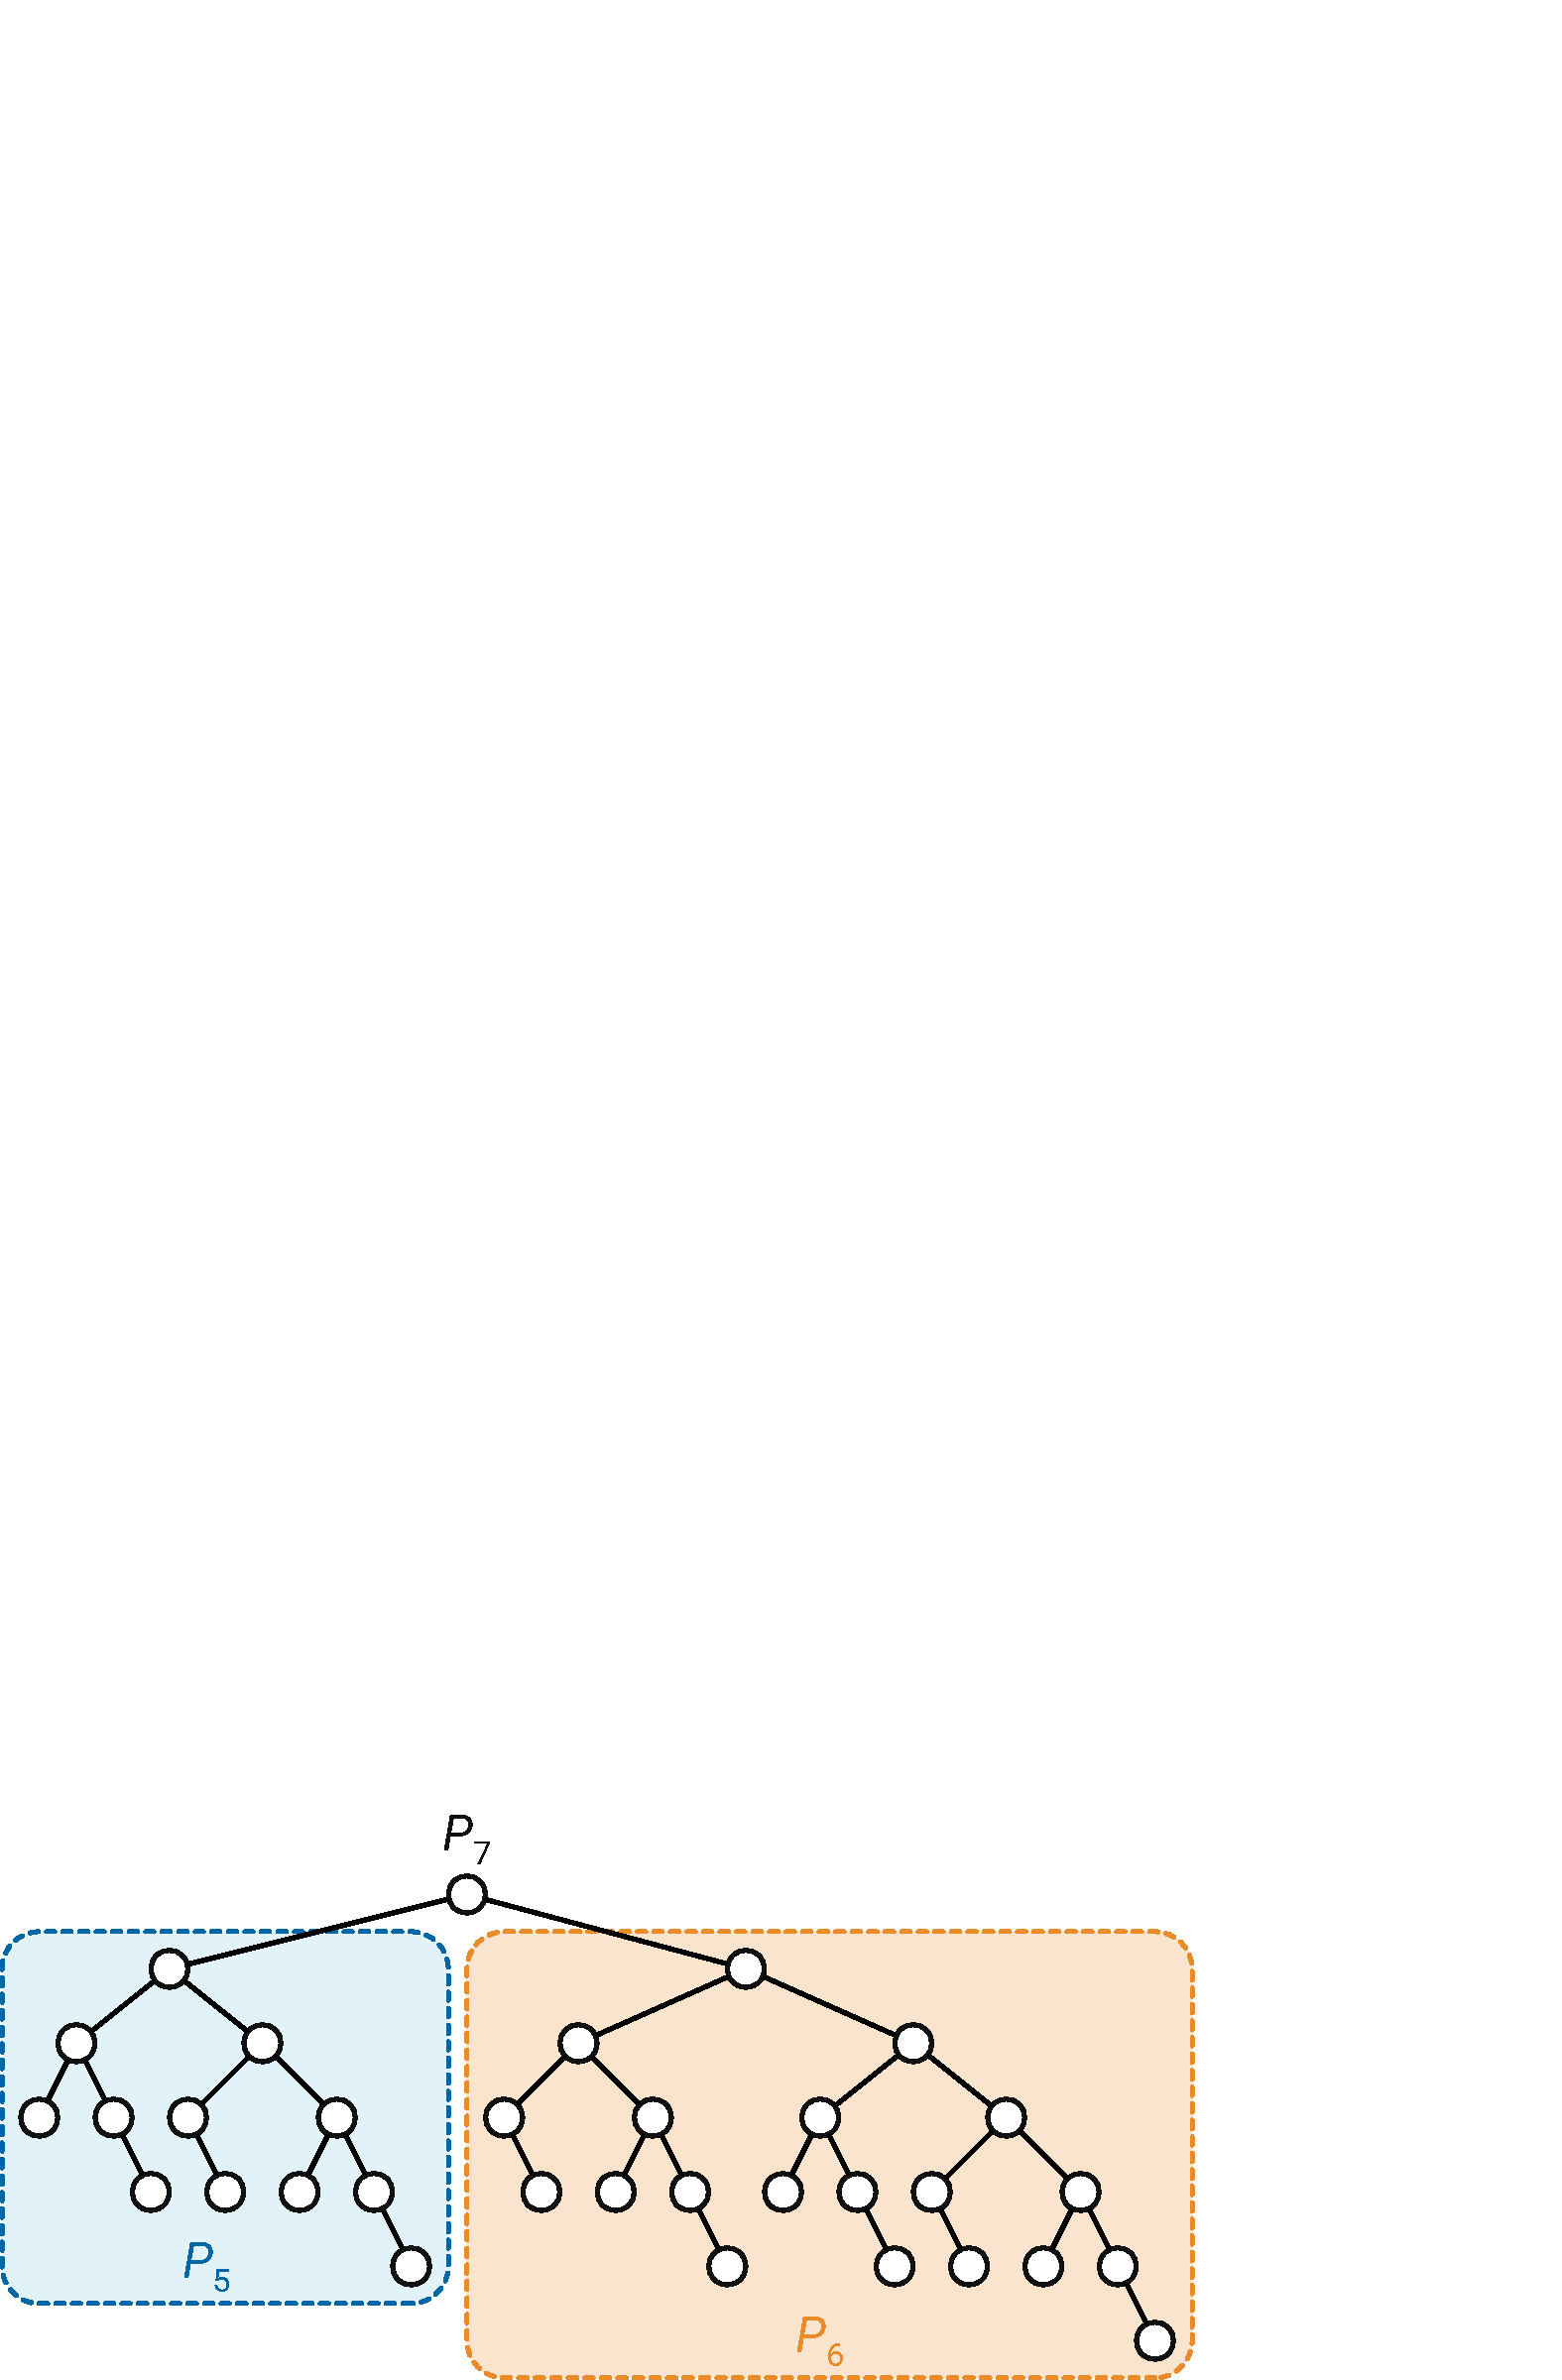
\includegraphics[scale=0.33,page=1]{Fig/fib-trees}\hfil
\includegraphics[scale=0.33,page=2]{Fig/fib-trees}
\end{center}

Recall that the Fibonacci numbers are defined recursively as follows:
\[
	F_n = \begin{cases}
		0 & \text{if $n=0$} \\
		1 & \text{if $n=1$} \\
		F_{n-1}+F_{n-2} & \text{otherwise}
	\end{cases}
\]
\begin{enumerate}
\item
Prove that the tree $P_n$ has exactly $F_n$ leaves.

\item
Prove that the tree $V_n$ has exactly $F_n$ leaves.

\Hint{You need to prove a stronger result.}

\item
Prove that the trees $P_n$ and $V_n$ are identical, for all $n\ge 0$.

\Hint{The hardest part of this proof is developing the right language/notation.}

\end{enumerate}

As in problem 1, you may freely use any result that proved in lecture, in lab, or in the lecture notes.  Otherwise your proofs must be formal and self-contained.  In particular, your proofs \emph{must} invoke the formal recursive definitions of the trees $P_n$ and $V_n$ and the Fibonacci numbers $F_n$.


\end{enumerate}
\newpage
%----------------------------------------------------------------------
\subsection*{Solved Problems}

\begin{enumerate}
\setcounter{enumi}{2}
%----------------------------------------------------------------------
\item
For any string $w \in \set{\Sym0,\Sym1}^*$, let $\emph{swap}(w)$ denote the string obtained from $w$ by swapping the first and second symbols, the third and fourth symbols, and so on.  For example:
\[
	\emph{swap}(\Sym{10\,11\,00\,01\,10\,1}) = \Sym{01\,11\,00\,10\,01\,1}.
\]
The \emph{swap} function can be formally defined as follows:
\[
	\emph{swap}(w) := \begin{cases}
		\e & \text{if $w=\e$}\\
		w & \text{if $w = \Sym0$ or $w = \Sym1$}\\
		ba\Cdot\emph{swap}(x) &
			\text{if $w = abx$ for some
					$a,b\in\set{\Sym0,\Sym1}$ and
					$x\in \set{\Sym0,\Sym1}^*$} 
	\end{cases}
\]

\begin{enumerate}
\item
Prove that $\abs{\emph{swap}(w)} = \abs{w}$ for every string $w$.

\begin{Solution}
\parindent0pt
Let $w$ be an arbitrary string.

Assume $\abs{\emph{swap}(x)} = \abs{x}$ for every string $x$ that is shorter than $w$.

There are three cases to consider (mirroring the definition of \emph{swap}):
\begin{itemize}
\item
If $w = \e$, then
\begin{align*}
	\abs{\emph{swap}(w)}
	&= \abs{\emph{swap}(\e)}	& \text{because $w = \e$} \\
	&= \abs{\e} 				& \text{by definition of \emph{swap}} \\
	&= \abs{w} 					& \text{because $w = \e$}
\end{align*}
\item
If $w = \Sym0$ or $w = \Sym1$, then
\begin{align*}
	\abs{\emph{swap}(w)}
	&= \abs{w} 					& \text{by definition of \emph{swap}}
\end{align*}
\item
Finally, if $w = abx$ for some $a,b\in\set{\Sym0,\Sym1}$ and $x\in\set{\Sym0,\Sym1}^*$ , then
\begin{align*}
	\abs{\emph{swap}(w)}
	&= \abs{\emph{swap}(abx)}			& \text{because $w = abx$} \\
	&= \abs{ba\Cdot\emph{swap}(x)}		& \text{by definition of \emph{swap}} \\
	&= \abs{ba} + \abs{\emph{swap}(x)}
										& \text{because $\abs{y\Cdot z} = \abs{y}+\abs{z}$}\\
	&= \abs{ba} + \abs{x}				& \text{by the induction hypothesis}\\
	&= 2 + \abs{x}						& \text{by definition of $\abs{\,\cdot\,}$}\\
	&= \abs{ab} + \abs{x}				& \text{by definition of $\abs{\,\cdot\,}$}\\
	&= \abs{ab\Cdot x}					& \text{because $\abs{y\Cdot z} = \abs{y}+\abs{z}$}\\
	&= \abs{abx} 						& \text{by definition of $\Cdot$}\\
	&= \abs{w} 							& \text{because $w = abx$}
\end{align*}
\end{itemize}
In all cases, we conclude that $\abs{\emph{swap}(w)} = \abs{w}$.
\end{Solution}
\unskip

\begin{rubric}
5 points: Standard induction rubric (scaled).  This is more detail than necessary for full credit.
\end{rubric}

\newpage
\item
Prove that $\emph{swap}(\emph{swap}(w)) = w$ for every string $w$.

\begin{Solution}
\parindent0pt
Let $w$ be an arbitrary string.

Assume $\emph{swap}(\emph{swap}(x)) = x$ for every string $x$ that is shorter than $w$.

There are three cases to consider (mirroring the definition of \emph{swap}):
\begin{itemize}
\item
If $w = \e$, then 
\begin{align*}
	\emph{swap}(\emph{swap}(w))
	&= \emph{swap}(\emph{swap}(\e))		& \text{because $w=\e$} \\
	&= \emph{swap}(\e)					& \text{by definition of \emph{swap}} \\
	&= \e								& \text{by definition of \emph{swap}} \\
	&= w								& \text{because $w=\e$}
\end{align*}
\item
If $w = \Sym0$ or $w = \Sym 1$, then 
\begin{align*}
	\emph{swap}(\emph{swap}(w))
	&= \emph{swap}(w)					& \text{by definition of \emph{swap}} \\
	&= w								& \text{by definition of \emph{swap}}
\end{align*}
\item
Finally, if $w = abx$ for some $a,b\in\set{\Sym0,\Sym1}$ and $x\in\set{\Sym0,\Sym1}^*$ , then
\begin{align*}
	\emph{swap}(\emph{swap}(w))
	&= \emph{swap}(\emph{swap}(abx))	& \text{because $w = abx$} \\
	&= \emph{swap}(ba\Cdot\emph{swap}(x))
										& \text{by definition of \emph{swap}} \\
	&= \emph{swap}(ba\Cdot z)
										& \text{where $z = \emph{swap}(x)$} \\
	&= \emph{swap}(baz)
										& \text{by definition of $\Cdot$} \\
	&= ab\Cdot \emph{swap}(z)
										& \text{by definition of \emph{swap}} \\
	&= ab\Cdot \emph{swap}(\emph{swap}(x))
										& \text{because $z = \emph{swap}(x)$} \\
	&= ab\Cdot x							& \text{by the induction hypothesis}\\
	&= abx 								& \text{by definition of $\Cdot$} \\
	&= w	 							& \text{because $w = abx$}
\end{align*}
\end{itemize}
In all cases, we conclude that $\emph{swap}(\emph{swap}(w)) = w$.
\end{Solution}
\unskip

\begin{rubric}
5 points: Standard induction rubric (scaled).  This is more detail than necessary for full credit.
\end{rubric}

\end{enumerate}

%----------------------------------------------------------------------
\newpage
\item
The \EMPH{reversal $w^R$} of a string $w$ is defined recursively as follows:
\[	
	w^R := \begin{cases}
		\e & \text{if $w=\e$} \\[0.5ex]
		x^R \Cdot a & \text{if $w=a\cdot x$}
	\end{cases}
\]
A \EMPH{palindrome} is any string that is equal to its reversal, like \Sym{AMANAPLANACANALPANAMA}, \hbox{\Sym{RACECAR}}, \Sym{POOP}, \Sym{I}, and the empty string.

\begin{enumerate}
\item
Give a recursive definition of a palindrome over the alphabet $\Sigma$.

\begin{Solution}
A string $w\in\Sigma^*$ is a palindrome if and only if either
\begin{itemize}
\item $w = \e$, or
\item $w = a$ for some symbol $a\in\Sigma$, or
\item $w = axa$ for some symbol $a\in\Sigma$ and some \emph{palindrome} $x\in\Sigma^*$.
\end{itemize}
\end{Solution}
\unskip
\begin{rubric}
2 points = \textonehalf\ for each base case + 1 for the recursive case.
No credit for the rest of the problem unless this part is correct.
\end{rubric}

\item
Prove $w = w^R$ for every palindrome $w$ (according to your recursive definition).  

You may assume the following facts about all strings $x$, $y$, and~$z$:
\begin{itemize}
\item Reversal reversal: $(x^R)^R = x$
\item Concatenation reversal: $(x\Cdot y)^R = y^R\Cdot x^R$
\item Right cancellation:  If $x\Cdot z = y\Cdot z$, then $x = y$.
\end{itemize}


\begin{Solution}
Let $w$ be an arbitrary palindrome.

Assume that $x = x^R$ for every palindrome $x$ such that $\abs{x}<\abs{w}$.

There are three cases to consider (mirroring the definition of “palindrome”):
\begin{itemize}
\item
If $w = \e$, then $w^R = \e$ by definition, so $w = w^R$.

\item
If $w = a$ for some symbol $a\in\Sigma$, then $w^R = a$ by definition, so $w = w^R$.

\item
Finally, if $w = axa$ for some symbol $a\in\Sigma$ and some palindrome $x\in P$, then 
\begin{align*}
	w^R
	&=	(a \cdot x \Cdot a)^R		& \text{because w = axa}\\
	&=	(x\Cdot a)^R \Cdot a			& \text{by definition of reversal} \\
	&=	a^R \Cdot x^R \Cdot a		& \text{by concatenation reversal}\\
	&=	a \Cdot x^R \Cdot a			& \text{by definition of reversal} \\
	&=	a \Cdot x \Cdot a			& \text{by the inductive hypothesis} \\
	&=	w							& \text{because w = axa}
\end{align*}
\end{itemize}
In all three cases, we conclude that $w = w^R$. \EOS
\end{Solution}
\unskip
\begin{rubric}
4 points: standard induction rubric (scaled)
\end{rubric}


\item
Prove that every string $w$ such that $w = w^R$ is a palindrome (according to your recursive definition).

Again, you may assume the following facts about all strings $x$, $y$, and~$z$:
\begin{itemize}
\item Reversal reversal: $(x^R)^R = x$
\item Concatenation reversal: $(x\Cdot y)^R = y^R\Cdot x^R$
\item Right cancellation:  If $x\Cdot z = y\Cdot z$, then $x = y$.
\end{itemize}


\begin{Solution}\parindent0pt
Let $w$ be an arbitrary string such that $w = w^R$.

Assume that every string $x$ such that $\abs{x} < \abs{w}$ and $x = x^R$ is a palindrome.

There are three cases to consider (mirroring the definition of “palindrome”):
\begin{itemize}\parskip0.25ex
\item 
If $w = \e$, then $w$ is a palindrome by definition.

\item 
If $w = a$ for some symbol $a\in\Sigma$, then $w$ is a palindrome by definition.

\item
Otherwise, we have $w = ax$ for some symbol $a$ and some \emph{non-empty} string~$x$.
  
The definition of reversal implies that $w^R = (ax)^R = x^R a$.

Because $x$ is non-empty, its reversal $x^R$ is also non-empty.

Thus, $x^R = by$ for some symbol $b$ and some string~$y$.

It follows that $w^R = bya$, and therefore $w = (w^R)^R = (bya)^R = a y^R b$.

\medskip
\Comment{At this point, we need to prove that $a=b$ and that $y$ is a palindrome.}
\medskip

Our assumption that $w = w^R$ implies that $bya = a y^R b$.

The recursive definition of string equality immediately implies $a=b$.

\medskip
Because $a=b$, we have $w = ay^Ra$ and $w^R = a y a$.

The recursive definition of string equality implies $y^Ra = ya$.

Right cancellation implies $y^R = y$.

The inductive hypothesis now implies that $y$ is a palindrome.

\medskip
We conclude that $w$ is a palindrome by definition.
\end{itemize}
In all three cases, we conclude that $w$ is a palindrome.\needqedtrue\EOS
\end{Solution}
\unskip
\begin{rubric}
4 points: standard induction rubric (scaled).
\end{rubric}

\end{enumerate}



\newpage
\item
Let $L \subseteq \set{\Sym0, \Sym1}^*$ be the language defined recursively as follows:
\begin{itemize}
\item
The empty string $\e$ is in $L$.
\item
For any string $x\in L$, the strings $\Sym{0101}x$ and $\Sym{1010}x$ are also in $L$.
\item
For all strings $x$ and $y$ such that $xy \in L$, the strings $x\Sym{00}y$ and $x\Sym{11}y$ are also in $L$.  (In other words, inserting two consecutive \Sym0s or two consecutive \Sym1s anywhere in a string in $L$ yields another string in $L$.)
\item
These are the only strings in $L$.
\end{itemize}

Let $EE$ denote the set of all strings $w \in \set{\Sym0, \Sym1}^*$ such that $\#(\Sym0,w)$ and $\#(\Sym1,w)$ are both even.

In the following proofs, you may freely use any result proved in lecture, in lab, in the lecture notes, or earlier in your homework.  Otherwise your proofs must be formal and self-contained; in particular, they must invoke the formal recursive definitions of $\#$ and $L$.


\begin{enumerate}
\item Prove that $L \subseteq EE$.

\begin{Solution}
Let $w$ be an arbitrary string in $L$.  We need to prove that $\#(\Sym0,w)$ and $\#(\Sym1,w)$ are both even.  Here I will prove only that $\#(\Sym0,w)$ is even; the proof that $\#(\Sym1,w)$ is even is symmetric.

Assume for every string $x\in L$ such that $\abs{x}<\abs{w}$ that $\#(\Sym0,x)$ is even.

There are several cases to consider, mirroring the definition of $L$.

\begin{itemize}
\item
Suppose $w = \e$.  Then $\#(\Sym0,w) = 0$, and $0$ is even.
\item
Suppose $w = \Sym{0101}x$ or $w = \Sym{1010}x$ for some string $x\in L$.  The  definition of $\#$ (applied four times) implies $\#(\Sym0, w) = \#(\Sym0, x) + 2$.  The inductive hypothesis implies $\#(\Sym0, x)$ is even.  We conclude that $\#(\Sym0, w)$ is even.

\item
Suppose $w = x\Sym{00}y$ for some strings $x$ and $y$ such that $xy\in L$.  Then
\begin{align*}
	\#(\Sym0, w) 
	&=
	\#(\Sym0, x\Sym{00}y) \\
	&=
	\#(\Sym0, x) + \#(\Sym0, \Sym{00}) + \#(\Sym0, y) \\
	&=
	\#(\Sym0, x) + \#(\Sym0, y) + \#(\Sym0, \Sym{00}) \\
	&=
	\#(\Sym0, xy) + 2
\end{align*}
The induction hypothesis implies $\#(\Sym0, xy)$ is even.  We conclude that $\#(\Sym0, w) = \#(\Sym0, xy) + 2$ is also even.

\item
Finally, suppose $w = x\Sym{11}y$ for some strings $x$ and $y$ such that $xy\in L$.  Then
\begin{align*}
	\#(\Sym0, w) 
	&=
	\#(\Sym0, x\Sym{11}y) \\
	&=
	\#(\Sym0, x) + \#(\Sym0, \Sym{11}) + \#(\Sym0, y) \\
	&=
	\#(\Sym0, x) + \#(\Sym0, y) \\
	&=
	\#(\Sym0, xy)
\end{align*}
The induction hypothesis implies $\#(\Sym0, w) = \#(\Sym0, xy)$ is even.
\end{itemize}
In all cases, we have shown that $\#(\Sym0, w)$ is even.  Symmetric arguments imply that $\#(\Sym1, w)$ is even.  We conclude that $w\in EE$.
\end{Solution}
\unskip
\begin{rubric}
5 points: standard induction rubric (scaled).  Yes, this is enough detail for $\#(\Sym1, w)$.  If explicit proofs are given for both $\#(\Sym0, w)$ and $\#(\Sym1, w)$, grade them independently, each for 2\textonehalf\ points.  
\end{rubric}

\medskip
\item Prove that $EE \subseteq L$.

\begin{Solution}\parindent 0pt
Let $w$ be an arbitrary string in $EE$.  We need to prove that $w\in L$.

Assume that for every string $x\in EE$ such that $\abs{x}<\abs{w}$, we have $x\in L$.

There are four (overlapping) cases to consider, depending on the first four symbols in $w$.
\begin{itemize}
\item
Suppose $\abs{w} < 4$.  Then $w$ must be one of the strings $\e$, $\Sym{00}$, or $\Sym{11}$; brute force inspection implies that every other string of length at most 3 (\Sym0, \Sym1, \Sym{01}, \Sym{10}, \Sym{000}, \Sym{001}, \Sym{010}, \Sym{011}, \Sym{100}, \Sym{101}, \Sym{110}, \Sym{111}) has an odd number of \Sym0s or an odd number of \Sym1s (or both).  All three strings $\e$, $\Sym{00}$, and $\Sym{11}$ are in $L$.  In all other cases, we can assume that $\abs{w} \ge 4$, so the “first four symbols of $w$” are well-defined.

\item
Suppose the first four symbols of $w$ are \Sym{00\underline{00}} or \Sym{0\underline{00}1} or \Sym{\underline{00}10} or \Sym{\underline{00}11} or \Sym{01\underline{00}} or \Sym{1\underline{00}0} or \Sym{1\underline{00}1} or \Sym{11\underline{00}}.  Then $w = x\Sym{00}y$ for some (possibly empty) strings $x$ and $y$.  Arguments in part (a) imply that $\#(\Sym0, xy) = \#(\Sym0, w) - 2$ and  $\#(\Sym1, xy) = \#(\Sym1, w)$ are both even.  Thus $xy\in EE$ by definition of $EE$.  So the induction hypothesis implies $xy\in L$.  We conclude that $w = x\Sym{00}y \in L$ by definition of $L$.

\item
Suppose the first four symbols of $w$ are \Sym{00\underline{11}} or \Sym{0\underline{11}0} or \Sym{0\underline{11}1} or \Sym{10\underline{11}} or \Sym{\underline{11}00} or \Sym{\underline{11}01} or \Sym{1\underline{11}0} or \Sym{\underline{11}11}.)  After swapping \Sym0s and \Sym1s, the argument in the previous case implies that $w \in L$.

\item
Finally, suppose the first four symbols of $w$ are \Sym{0101} or \Sym{1010}; in other words, suppose $w = \Sym{0101}x$ or $w = \Sym{1010}x$ for some (possibly empty) string $x$.  Then $\#(\Sym0, x) = \#(\Sym0, w) - 2$ and $\#(\Sym1, x) = \#(\Sym1, w) - 2$ are both even, so $x\in EE$ by definition.  The induction hypothesis implies $x\in L$.  We conclude that $w \in L$ by definition of $L$.

\end{itemize}
Each of the 16 possible choices for the first four symbols of $w$ is considered in at least one of the last three cases.

In all cases, we conclude that $w \in L$.
\end{Solution}
\unskip
\begin{rubric}
5 points: standard induction rubric (scaled).  This is not the only correct proof.  This is not the only correct  way to express this particular case analysis.
\end{rubric}


\end{enumerate}



\end{enumerate}


\end{document}
